% Anonymous Credentials from SD-JWT VC -- working draft (skeleton).
% Merged from the markdown section drafts in the repo root:
%   paper-introduction-draft.md  -> Abstract + Sec 1
%   (background stub)            -> Sec 2
%   paper-security-draft.md      -> Sec 3 (threat model) + Sec 5 (security)
%   paper-construction-draft.md  -> Sec 4
%   paper-evaluation-draft.md    -> Sec 7
%   paper-related-work-draft.md  -> Sec 8 + Table 1
% Portable preamble (compiles with a vanilla TeX Live, pdflatex).
% To target PoPETs/ACM later, swap \documentclass for the venue class.

\documentclass[11pt]{article}

\usepackage[utf8]{inputenc}
\usepackage[T1]{fontenc}
\usepackage[margin=1in]{geometry}
\usepackage{amsmath,amssymb,amsthm}
\usepackage{booktabs}
\usepackage{graphicx}
\usepackage{pifont}      % \ding for check/cross marks
\usepackage{xcolor}
\usepackage{tikz}
\usetikzlibrary{arrows.meta,positioning,fit,backgrounds,calc}
\usepackage[hidelinks]{hyperref}
\usepackage{microtype}
\setlength{\emergencystretch}{1em}

% comparison-table marks
\newcommand{\cmark}{\ding{51}}          % yes
\newcommand{\xmark}{\ding{55}}          % no
\newcommand{\pmark}{$\sim$}             % partial
\newcommand{\TODO}[1]{\textcolor{red}{[\textbf{TODO:} #1]}}

\theoremstyle{plain}
\newtheorem{theorem}{Theorem}
\theoremstyle{definition}
\newtheorem{definition}[theorem]{Definition}

\title{Anonymous Credentials from SD-JWT VC:\\
Issuer-Unlinkable Nullifiers and Revocation in Transparent Zero-Knowledge}
\author{Anonymous Submission\thanks{Author block withheld for review.}}
\date{}

\begin{document}
\maketitle

\begin{abstract}
Selective-disclosure credentials---IETF \emph{SD-JWT VC} and \emph{ISO mdoc}---are
being deployed at national scale in digital identity wallets, yet they provide
\emph{no unlinkability}: a static issuer signature over static salted hashes lets
colluding verifiers, and the issuer itself, correlate a user's presentations. The
only standardized mitigation, \emph{batch issuance}, provides verifier-unlinkability
only and at a recurring per-presentation cost. We turn \emph{unmodified} SD-JWT VC
and mdoc credentials into anonymous credentials using \textbf{transparent,
no-trusted-setup zero-knowledge}. Our framework unifies selective disclosure,
attribute predicates, an \textbf{issuer-unlinkable per-context blind nullifier}, and
signed-range non-membership revocation over both formats. The blind nullifier is, to
our knowledge, the first that binds to an issuer-signed standard credential,
\emph{never de-anonymizes} its holder, and is \emph{publicly verifiable} in
transparent zero-knowledge---unlike PLUME/Semaphore nullifiers, Privacy Pass/ARC
rate-limit tags, and e-cash double-spend tags. Implemented on longfellow-zk, a
presentation proves in under 2\,s and verifies in under 0.85\,s on commodity hardware
($\approx$1.0\,s\,/\,0.45\,s for mdoc), with no trusted setup and no change to issuers
or devices; issuer-untraceability costs under 5\% over a plain nullifier.
\end{abstract}

% =====================================================================
\section{Introduction}\label{sec:intro}

Digital identity wallets are moving from pilots to law. The European Digital
Identity (eIDAS~2.0) framework obliges member states to offer wallets to all
citizens~\cite{eidas2}, and mobile driver's licenses (mDL) are rolling out across
U.S.\ states~\cite{aamva-mdl}. Two credential formats dominate these deployments:
\textbf{IETF SD-JWT VC}~\cite{sdjwtvc}, a JSON/JWS credential with salted-hash
selective disclosure, and \textbf{ISO/IEC 18013-5 mdoc}~\cite{iso18013}, its CBOR
counterpart. Both let a holder reveal a subset of attributes (e.g., \emph{age
$\geq$ 18}) while hiding the rest.

\paragraph{The problem: selective disclosure is not unlinkability.}
Hiding \emph{which} attributes are shown does not hide \emph{who} is showing them.
In both formats the issuer signs a fixed set of salted attribute hashes, and the
holder forwards that issuer signature, verbatim, to every relying party. The
signature and the salted hashes are therefore stable identifiers: any two relying
parties that compare notes---or the issuer colluding with a relying party---can link
a user's interactions, and the issuer, who produced the signature, can recognize it
anywhere. A standards-body taxonomy makes the distinction explicit, separating
\emph{verifier}-unlinkability from full \emph{issuer}-unlinkability and noting that
the salted-hash formats provide neither natively~\cite{etsi119476}. A statement
signed by sixteen cryptographers warned the EU that this design ``cannot ensure
unlinkability,'' which eIDAS~2.0 lists as a mandatory requirement~\cite{eudi-crypto-feedback}.

\paragraph{The state of practice is unsatisfying.}
The only mitigation standardized today---across OpenID4VCI, RFC~9901, the
High-Assurance Interoperability Profile, and the EUDI reference
framework~\cite{openid4vci,rfc9901,haip,eudi-arf}---is \emph{batch issuance}: the
issuer mints many single-use credentials, each with fresh salts and key-binding
keys, and the holder spends one per presentation. This buys only
\emph{verifier}-unlinkability---the issuer can still correlate---at a recurring cost
in issuance, storage, and key management, and it fails outright once a credential is
reused. Cryptographic alternatives exist but each asks issuers to abandon their
deployed credential: BBS\#-style anonymous-credential signatures~\cite{bbs-sharp2025}
require a new signature scheme (and issuer assistance at presentation), while
SNARK-based systems that prove possession of an existing
credential---Crescent~\cite{paquin2024crescent}, zk-creds~\cite{rosenberg2023zkcreds}---depend
on a circuit-specific \emph{trusted setup} whose compromise silently breaks
soundness. None of these targets the SD-JWT VC format that wallets are actually
shipping.

\paragraph{Our approach.}
We make \emph{unmodified} SD-JWT VC and ISO mdoc credentials unlinkable by proving
their possession in \textbf{transparent zero-knowledge}---an argument system
(Ligero~+~sumcheck) that needs no common reference string and rests only on SHA-256,
building on longfellow~\cite{frigo2024longfellow}. The issuer keeps signing ordinary
ECDSA credentials; the holder, at presentation, produces a proof that reveals only
the attributes it chooses, the truth of a predicate, a per-context pseudonymous tag,
and an epoch-fresh non-revocation fact---nothing else, and to no one, including the
issuer. Within this framework we contribute the missing primitive that batch
issuance and prior ZK systems lack: a nullifier that even the issuer cannot trace.

\paragraph{An issuer-unlinkable blind nullifier.}
A nullifier is a per-context tag that lets a verifier detect repeat use (one vote per
election, one account per service) without identifying the holder. Existing
constructions either reveal the holder on reuse (e-cash, zk-creds clone-resistance),
are computed from a self-held key with no issuer-signed credential behind them (PLUME,
Semaphore), or are privately verifiable so the issuer is a co-verifier (Privacy
Pass/ARC). We instead have the \emph{holder} commit a secret $s$ at
issuance---$C=\mathsf{SHA256}(s\|r)$, which the issuer signs as an ordinary disclosure
without ever seeing $s$---and derive the per-context nullifier
$N=\mathsf{SHA256}(s\|\mathit{ctx})$ inside the proof, binding $N$ to the same $s$ the
credential committed to. Because the issuer's only view of the seed is the hiding
commitment $C$, it cannot recompute or recognize $N$: the nullifier is
\emph{issuer-untraceable} (Theorem~\ref{thm:untrace}). To our knowledge this is the
first issuer-unlinkable nullifier bound to an unmodified, publicly verifiable standard
credential, and---being SHA-256 throughout---it adds no cryptographic assumption
beyond the base proof system.

\paragraph{Contributions.}
\begin{itemize}
\item \textbf{(C1)} The first transparent, no-trusted-setup zero-knowledge
construction over the \textbf{unmodified IETF SD-JWT VC} format---new circuits for its
JSON/JWS/base64url/salted-hash structure---generalized to ISO mdoc through a shared
seam (\S\ref{sec:construction}).
\item \textbf{(C2)} An \textbf{issuer-unlinkable per-context blind nullifier} bound to
a standard credential, with a security definition and proof of issuer-untraceability
(\S\ref{sec:security}), and a precise separation from PLUME, Semaphore, Privacy
Pass/ARC, and e-cash (\S\ref{sec:related}).
\item \textbf{(C3)} A \textbf{single framework} unifying selective disclosure,
attribute predicates, the blind nullifier, and signed-range non-membership revocation
over \emph{both} SD-JWT VC and mdoc (\S\ref{sec:construction}). We adopt the
signed-range revocation \emph{mechanism} from longfellow and contribute its extension
to SD-JWT VC and its integration.
\item \textbf{(C4)} An \textbf{implementation} on longfellow-zk and an evaluation
showing the system runs with no issuer/device changes and no trusted setup, at
practical cost (\S\ref{sec:eval}).
\end{itemize}

\paragraph{Results.}
On a commodity desktop, every configuration proves in under 2\,s and verifies in
under 0.85\,s ($\approx$1.0\,s\,/\,0.45\,s for mdoc), with $\approx$390\,KB (SD-JWT VC)
and $\approx$350\,KB (mdoc) proofs. The issuer-untraceable blind nullifier costs under
5\% over a plain nullifier with no increase in proof size, and signed-range revocation
adds a constant overhead independent of the revocation-list size. We also quantify,
for the first time, the in-circuit cost of SD-JWT VC's text encoding: its
base64url/JSON parsing roughly doubles the hash-circuit work relative to mdoc's CBOR.

% =====================================================================
\section{Background}\label{sec:background}
We recall the two credential formats, the linkability notion we target, and the
transparent argument we build on.

\paragraph{SD-JWT VC.} A JWS over a payload carrying \texttt{\_sd}, an array of
disclosure digests, and a holder-binding key in \texttt{cnf}; each disclosure is
$\mathsf{base64url}(\mathrm{JSON}([\mathit{salt},\mathit{name},\mathit{value}]))$ bound
by $\mathsf{SHA256}(\text{disclosure})\in\texttt{\_sd}$.

\paragraph{ISO mdoc.} A CBOR credential whose Mobile Security Object signs salted
device-namespace attribute hashes under ECDSA-P256.

\paragraph{Linkability model.} Following~\cite{etsi119476} we distinguish
\emph{verifier}-unlinkability (relying parties cannot correlate) from
\emph{issuer}-unlinkability (the issuer cannot correlate); \emph{full} unlinkability
requires both.

\paragraph{Transparent zero-knowledge.} longfellow~\cite{frigo2024longfellow,libzk-draft}
combines the Ligero MPC-in-the-head argument with a sumcheck verifiable-computation
protocol; it has \emph{no common reference string} and relies only on SHA-256, with
Fiat--Shamir in the random-oracle model.

% =====================================================================
\section{Threat Model and Security Goals}\label{sec:threat}

\subsection{System model and parties}
The system has three roles. An \textbf{issuer} $\mathcal{I}$ holds a signing key
$(\mathit{isk},\mathit{ipk})$ and issues standard credentials (SD-JWT VC or mdoc) by
signing a set of salted attribute hashes together with a holder-binding public key. A
\textbf{holder} $\mathcal{H}$ stores a credential and acts as prover. A
\textbf{verifier} $\mathcal{V}$ checks a presentation against a public statement
(disclosed attributes, a predicate $\phi$, a presentation context $\mathit{ctx}$, and
current revocation information). Revocation information is published by a
\textbf{certificate-revocation authority} $\mathcal{C}$ (possibly $\mathcal{I}$) as
signed \emph{gaps} between adjacent revoked identifiers. A \textbf{presentation
context} $\mathit{ctx}$ is a public string scoping a nullifier; the nullifier is
per-context.

\subsection{Trust and adversary model}
\begin{itemize}
\item \textbf{No trusted setup.} The scheme is transparent: the only public
parameters are a collision-resistant hash $H$ (SHA-256, modeled as a random oracle for
Fiat--Shamir) and a commitment scheme. There is no common reference string and hence
no toxic waste; soundness rests on no party having to honestly discard a trapdoor.
This is the central distinction from Groth16-based schemes, whose soundness
additionally requires the integrity of a circuit-specific setup.
\item \textbf{Issuer.} Honest at issuance but treated as an adversary for
unlinkability: it may later collude with verifiers and use everything it observed at
issuance, including the blind-nullifier commitments it signed. Its signing key is not
compromised.
\item \textbf{Verifiers.} May be malicious and may collude with one another and with
the issuer.
\item \textbf{Holder.} A malicious holder may try to forge a presentation, satisfy a
predicate it does not, or present twice under one context with distinct nullifiers.
\item Channels are confidential; the holder-binding key is held in a secure element
and proven in zero knowledge, never revealed.
\end{itemize}

\subsection{Security goals (informal)}\label{sec:goals}
\begin{enumerate}
\item \textbf{Completeness.}
\item \textbf{Soundness / credential unforgeability.}
\item \textbf{Selective-disclosure zero-knowledge.}
\item \textbf{Unlinkability} (verifier and issuer).
\item \textbf{Nullifier determinism \& uniqueness.}
\item \textbf{Issuer-untraceability of the nullifier} ($\star$).
\item \textbf{Revocation soundness \& privacy.}
\end{enumerate}

\paragraph{Uniqueness scope and issuance assumption.}
Goal~5 is \emph{per credential}: one credential yields one nullifier per context.
Because issuance is blind, the issuer never sees the seed $s$ and cannot enforce that a
person holds only one, so a holder with $k$ credentials produces $k$ independent
nullifiers. Sybil-resistance applications (e.g., one vote per election) therefore rest
on the standard assumption that the issuer issues \emph{one credential per
person}---an identified, out-of-band step the issuer already controls---after which
per-credential uniqueness \emph{is} per-person uniqueness and the nullifier
deduplicates that credential's re-presentations within a context. Making $s$
person-unique without the issuer learning it (e.g., deriving $s$ in the secure element,
or an issuer-side deterministic tag proven equal to $s$ in zero-knowledge) is an
alternative we leave to future work.

% =====================================================================
\section{Construction}\label{sec:construction}

\subsection{Overview}
Our prover convinces a verifier, in transparent zero-knowledge, that it holds an
issuer-signed standard credential satisfying a public statement, while revealing only
the disclosed attributes, the truth of a predicate, a per-context nullifier, and an
epoch-pinned non-revocation fact. We build on longfellow's transparent argument
(Ligero~+~sumcheck, SHA-256 only) and its \emph{split-circuit} architecture, which we
(i)~drive from the IETF SD-JWT VC wire format, (ii)~extend with an issuer-unlinkable
blind nullifier, and (iii)~combine with signed-range non-membership revocation---the
same three feature blocks running unmodified over ISO mdoc through a shared seam
(\S\ref{sec:unify}). Every gadget is expressed in SHA-256 and P-256 ECDSA, so no
assumption beyond longfellow's is introduced.

\subsection{Split-circuit seam}\label{sec:seam}
Proving ECDSA and SHA-256 in a single field is wasteful: ECDSA arithmetic lives in
the P-256 base field $\mathbb{F}_p$, whereas SHA-256's bit operations are cheap over
$\mathrm{GF}(2^{128})$. Following longfellow, we use \emph{two circuits in their native
fields}---a signature circuit over $\mathbb{F}_p$ that verifies the issuer's ECDSA
signature, and a hash circuit over $\mathrm{GF}(2^{128})$ that recomputes the SHA-256
structure---\emph{linked by a MAC} over the values they share: $e$ (the digest the
issuer signs), $\mathit{dpk}_x,\mathit{dpk}_y$ (the holder-binding key), and, with
revocation, $e_{\mathrm{span}}$. The prover commits its half $a_p$ of a
$\mathrm{GF}(2^{128})$ MAC key and the shared values \emph{before} the Fiat--Shamir
challenge reveals $a_v$; the resulting MACs are public inputs to both circuits. By
Schwartz--Zippel, a prover cannot feed two different values to the two circuits except
with negligible probability. This seam is shared by all feature configurations
(Figure~\ref{fig:seam}).

\begin{figure}[t]\centering
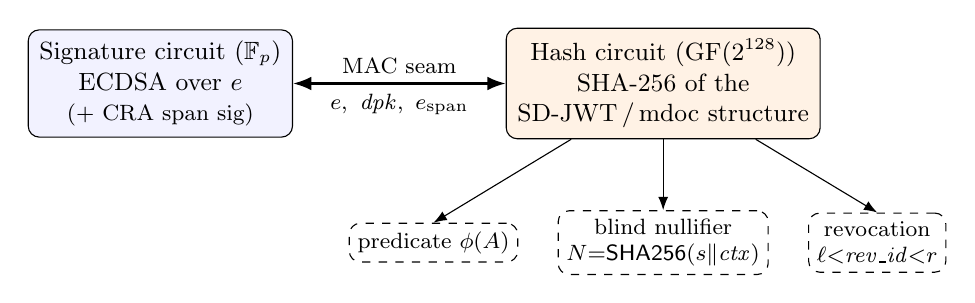
\begin{tikzpicture}[
  font=\small, >=Latex,
  box/.style={draw, rounded corners, align=center, minimum height=1.15cm, inner sep=4pt},
  feat/.style={draw, dashed, rounded corners, align=center, font=\footnotesize, inner sep=3pt}]
  \node[box, fill=blue!5] (sig) {Signature circuit $(\mathbb{F}_p)$\\ ECDSA over $e$\\ {\footnotesize(+ CRA span sig)}};
  \node[box, fill=orange!10, right=2.7cm of sig] (hash) {Hash circuit $(\mathrm{GF}(2^{128}))$\\ SHA-256 of the\\ SD-JWT\,/\,mdoc structure};
  \draw[<->, thick] (sig) -- node[above, font=\footnotesize]{MAC seam}
                            node[below, font=\footnotesize]{$e,\ \mathit{dpk},\ e_{\mathrm{span}}$} (hash);
  \node[feat, below=0.9cm of hash] (null) {blind nullifier\\ $N{=}\mathsf{SHA256}(s\|\mathit{ctx})$};
  \node[feat, left=0.5cm of null] (pred) {predicate $\phi(A)$};
  \node[feat, right=0.5cm of null] (rev) {revocation\\ $\ell{<}\mathit{rev\_id}{<}r$};
  \draw[->] (hash) -- (pred.north); \draw[->] (hash) -- (null); \draw[->] (hash) -- (rev.north);
\end{tikzpicture}
\caption{Split-circuit architecture. A signature circuit $(\mathbb{F}_p)$ and a hash
circuit $(\mathrm{GF}(2^{128}))$ are linked by a MAC over the shared values
$e,\mathit{dpk},e_{\mathrm{span}}$; the format-agnostic feature blocks (predicate,
issuer-unlinkable blind nullifier, signed-range revocation) attach to the hash circuit
and run unchanged for SD-JWT VC and mdoc.}
\label{fig:seam}
\end{figure}

\subsection{SD-JWT VC front-end}\label{sec:frontend}
The signature circuit verifies \emph{two} ECDSA signatures: the issuer's ES256 over
the payload digest $e$, and the holder's key-binding-JWT signature over its digest
$e_2$ under the device key $\mathit{dpk}$. The hash circuit recomputes, in-circuit:
(a)~the SD-JWT structure and $e$, (b)~for each presented disclosure, its base64url
decoding and membership of its digest in \texttt{\_sd}, and (c)~the key-binding JWT
payload (its digest $e_2$, and the verifier's \texttt{nonce}/\texttt{aud}). Each
requested claim is handled in one of two modes: \emph{disclose}---the value is matched
against a public pattern and revealed---or \emph{assert}---the value stays hidden and
only a \emph{predicate} over it (range, equality, set membership) is enforced. The
device key $\mathit{dpk}$ is checked in-circuit to equal the issuer-attested
\texttt{cnf} key, and the holder's signature over $e_2$ is verified (but, like
$\mathit{dpk}$ itself, never revealed): a valid presentation therefore \emph{requires
the holder's secure-element key} (\S\ref{sec:relation}) while leaking no linkable
handle.

\subsection{Issuer-unlinkable blind nullifier}\label{sec:blind}
This is our central construction. The goal is a per-context tag $N$ that is unique per
credential within a context, unlinkable across contexts, and untraceable even by the
issuer.

\paragraph{Issuance (blind).} The \emph{holder} samples a 256-bit seed $s$ and a
256-bit blind $r$ and forms a hash commitment $C=\mathsf{SHA256}(s\|r)$. The issuer
signs $C$ as an ordinary disclosure (\texttt{pseudonym\_commitment}) included in
\texttt{\_sd}; it commits to $C$---the holder cannot later swap it---\emph{yet never
observes $s$ or $r$}.

\paragraph{Presentation.} For a verifier-chosen context the prover takes
$\mathit{ctx\_hash}=\mathsf{SHA256}(\mathit{ctx})$ as a public input and proves, in
zero-knowledge:
\begin{enumerate}
\item \emph{membership} --- $\mathsf{SHA256}(\text{commitment disclosure})\in\texttt{\_sd}$;
\item \emph{structure} --- the disclosure decodes to the JSON triple \texttt{[salt, "pseudonym\_commitment", C]};
\item \emph{decoding} --- the base64url value decodes to the 32-byte $C$;
\item \emph{opening} --- $\mathsf{SHA256}(s\|r)$ equals $C$;
\item \emph{nullifier} --- $N=\mathsf{SHA256}(s\|\mathit{ctx\_hash})$, from the \emph{same $s$ wires} as the opening.
\end{enumerate}
The only public outputs are $\mathit{ctx\_hash}$ and $N$; the commitment, disclosure,
seed, and blind remain hidden. Sharing the $s$ wires between steps~4 and~5 binds the
value the issuer committed to exactly the value inside the nullifier.

\paragraph{Why this is issuer-untraceable.} The issuer's entire view of the seed is
the hiding commitment $C=\mathsf{SHA256}(s\|r)$; with a 256-bit random $r$ and SHA-256
modeled as a random oracle, $C$ reveals nothing about $s$, so $N$ is pseudorandom from
the issuer's view (Theorem~\ref{thm:untrace}). Because both the commitment and the
nullifier are SHA-256, the blind nullifier adds \emph{no} assumption beyond
longfellow's. This distinguishes it from PLUME/Semaphore (no issuer-signed credential),
ARC (privately verifiable), and e-cash serial numbers (de-anonymize on reuse);
see~\S\ref{sec:related}.

\subsection{Signed-range non-membership revocation}\label{sec:revoc}
We adopt longfellow's signed-range mechanism and extend it to SD-JWT VC; we claim the
\emph{extension and integration}, not the mechanism. A revocation authority sorts the
revoked identifiers and signs the open gaps between adjacent revoked ids as spans
$\mathit{epoch}\|\ell\|r$. The credential carries a hidden \texttt{revocation\_id}
(its \texttt{\_sd} digest $\mathit{rev\_id}$). To prove non-revocation the holder
presents one signed span with $\ell<\mathit{rev\_id}<r$. In-circuit, the CRA's ECDSA
signature over $e_{\mathrm{span}}=\mathsf{SHA256}(\mathit{epoch}\|\ell\|r)$ is verified
in the signature circuit; $e_{\mathrm{span}}$ is bound to the hash circuit by a fourth
MAC; $\mathit{epoch}$ is a public freshness pin; and $\ell<\mathit{rev\_id}<r$ is
checked bitwise. The proof size is \emph{constant regardless of the revocation-list
size} and reveals neither $\mathit{rev\_id}$ nor which gap was used.

\subsection{Unification across SD-JWT VC and mdoc}\label{sec:unify}
The seam and feature blocks are format-agnostic: they operate on the shared values and
issuer-committed digests, not on the surface encoding. Only the front-end
differs---SD-JWT VC parses JWS/base64url/\texttt{\_sd}, whereas mdoc parses
CBOR/MSO/salted hashes. Consequently the blind-nullifier and revocation blocks are
identical across formats, and one shared implementation is the source of truth for
both. Table~\ref{tab:checks} makes this concrete: the two formats verify the
\emph{same} in-circuit checks---including the device-key signature that binds each
presentation to the holder's secure element---and differ only in parsing, which is also
the source of the runtime gap (\S\ref{sec:eval}).

\begin{table}[t]\centering\small
\caption{What the circuit verifies, by format. The checks are identical; only the
parsing front-end differs.}
\label{tab:checks}
\begin{tabular}{@{}lll@{}}
\toprule
Check & SD-JWT VC & ISO mdoc \\
\midrule
Issuer ECDSA              & over JWS hash $e$              & over MSO hash $e$ \\
Device ECDSA (holder)     & KB-JWT over $e_2$             & session transcript over $e_2$ \\
Device key attested       & $\mathit{dpk}=\mathtt{cnf}$   & $\mathit{dpk}=\mathtt{deviceKey}$ \\
Disclosure membership     & digest $\in\mathtt{\_sd}$     & digest $\in\mathtt{valueDigests}$ \\
Predicate / nullifier / revocation & \multicolumn{2}{c}{identical feature blocks} \\
\midrule
Parsing front-end         & JWS, base64url, JSON          & CBOR, MSO \\
\bottomrule
\end{tabular}
\end{table}

\subsection{The full presentation}
A complete presentation bundles the signature- and hash-circuit proofs (and, with
revocation, the CRA span proof) with the public statement
$x=(\mathit{ipk},\mathit{ctx\_hash},N,D,\phi,\mathit{rinfo})$ of \S\ref{sec:relation},
establishing all clauses of the relation $\mathcal{R}$ with no trusted setup.

% =====================================================================
\section{Implementation}\label{sec:impl}
We implement the system in C++ on top of longfellow-zk. A single shared header is the
source of truth for the split-circuit seam (\S\ref{sec:seam})---the MAC machinery, the
public-input layout, and the compiled-circuit cache---while a thin per-format front-end
parses SD-JWT VC or mdoc and each feature is an additive circuit block. The four
configurations per format (base, nullifier, blind nullifier, revocation) thus share one
codebase, and the SD-JWT VC and mdoc variants differ only in their front-end. ECDSA
verification reuses longfellow's P-256 circuit and SHA-256 its flat-witness gadget, so
the blind nullifier's commitment and tag reduce to two extra SHA-256 blocks
(\S\ref{sec:blind}). Circuits are compiled once and cached (zstd-compressed) so that
proving and verification do not pay the build cost. An evaluation harness regenerates
the issuer/holder fixtures and records the numbers reported in \S\ref{sec:eval}.

% =====================================================================
\section{Security Analysis}\label{sec:security}

\subsection{Building blocks and assumptions}
\begin{itemize}
\item \textbf{Issuer signature} $\mathsf{Sig}$ over the credential (ECDSA-P256),
EUF-CMA (ECDSA in GGM+ROM).
\item \textbf{Commitment} $\mathsf{COM}$, computationally hiding and binding,
\emph{instantiated as a SHA-256 hash commitment} $C=\mathsf{SHA256}(s\|r)$ with a
256-bit blind (\S\ref{sec:blind}): hiding holds in the ROM, binding by collision
resistance---so it adds no assumption beyond longfellow's.
\item \textbf{Nullifier hash} $H_{\mathsf{nul}}$: $N=H_{\mathsf{nul}}(s,\mathit{ctx})$,
a random oracle / PRF keyed by $s$.
\item \textbf{Transparent argument} $\mathsf{NIZK}$ (Ligero~+~sumcheck, Fiat--Shamir
in the ROM), knowledge-sound and zero-knowledge, no setup.
\item \textbf{CRA signature} for revocation gaps, EUF-CMA.
\end{itemize}

\subsection{The presentation relation}\label{sec:relation}
A presentation is a $\mathsf{NIZK}$ for the relation $\mathcal{R}$ on public statement
$x=(\mathit{ipk},\mathit{ctx},N,D,\phi,\mathit{rinfo})$ and witness
$w=(\mathit{cred},\sigma,\sigma_{\mathrm{kb}},\mathit{dpk},s,r,A,\pi_{\mathrm{rev}})$.
$\mathcal{R}(x,w)=1$ iff:
\begin{enumerate}
\item $\mathsf{SigVer}(\mathit{ipk},\mathit{cred},\sigma)=1$ --- valid issuer signature
over the unmodified standard credential;
\item \emph{(device binding)} $\mathsf{SigVer}(\mathit{dpk},e_2,\sigma_{\mathrm{kb}})=1$
and $\mathit{dpk}$ equals the holder-binding key the issuer attested in $\mathit{cred}$
(\texttt{cnf} for SD-JWT VC, \texttt{deviceKey} for mdoc), where $e_2$ binds the
presentation session (the KB-JWT, resp.\ the session transcript); a valid presentation
therefore requires the device's secure-element key;
\item a signed attribute equals $C=\mathsf{Commit}(s;r)$;
\item $N=H_{\mathsf{nul}}(s,\mathit{ctx})$;
\item $D$ is consistent with $\mathit{cred}$ and $A\supseteq D$;
\item $\phi(A)=1$;
\item $\ell<\mathit{rev\_id}<r$ for a CRA-signed gap $(\ell,r)$ in $\mathit{rinfo}$.
\end{enumerate}
The statement reveals only $N$ and $\mathit{ctx}$ (plus $D,\phi,\mathit{rinfo}$);
$\sigma$, $C$, $s$, $r$, the holder-binding key, $\mathit{rev\_id}$, and the chosen gap
remain hidden.

\subsection{Definitions and theorems}
We state each property as a game; $\mathsf{negl}$ is negligible in the security
parameter $\lambda$. Proof sketches are given here; the two load-bearing games
(credential soundness and issuer-untraceability) are restated in pseudocode with
fuller proofs in Appendix~\ref{app:proofs}.

\begin{theorem}[Completeness]\label{thm:complete}
If $\mathit{cred}$ is validly issued, non-revoked, and satisfies $(D,\phi)$, an honest
prover convinces the verifier with probability $1-\mathsf{negl}(\lambda)$.
\end{theorem}
\begin{proof}[Proof sketch] Immediate from completeness of $\mathsf{NIZK}$. \end{proof}

\begin{definition}[Credential soundness]\label{def:sound}
$\mathcal{A}$ gets $\mathit{ipk}$ and an $\mathsf{Issue}$ oracle (recording $Q$); it
wins if it outputs an accepting $(x^*,\pi^*)$ for which no issued $\mathit{cred}\in Q$
both carries a valid signature and is consistent with $x^*$.
\end{definition}
\begin{theorem}\label{thm:sound}
If $\mathsf{NIZK}$ is knowledge-sound, $\mathsf{Sig}$ is EUF-CMA, and $\mathsf{COM}$ is
binding, then $\Pr[\mathcal{A}\text{ wins}]\le\mathsf{negl}(\lambda)$.
\end{theorem}
\begin{proof}[Proof sketch] The extractor yields $(\mathit{cred}^*,\sigma^*,s^*,r^*)$
with $\mathcal{R}(x^*,\cdot)=1$; if $\mathit{cred}^*\notin Q$ this is an EUF-CMA
forgery, otherwise consistency clauses (bound via the signature and commitment
binding) contradict the win condition. \end{proof}

\begin{definition}[Selective-disclosure ZK]\label{def:zk}
There is a simulator $\mathsf{Sim}$ such that for every valid $(x,w)$, no PPT
$\mathcal{A}$ distinguishes $\mathsf{Prove}(x,w)$ from $\mathsf{Sim}(x)$.
\end{definition}
\begin{theorem}\label{thm:zk}
Follows from zero-knowledge of $\mathsf{NIZK}$: a presentation is one proof for $x$, so
it leaks nothing beyond $x$.
\end{theorem}

\begin{definition}[Verifier-unlinkability]\label{def:vunlink}
In a left-or-right game $\mathcal{A}$ (colluding verifiers) chooses two non-revoked
credentials equivalent on the challenge statement (same $D$, same $\phi(A)$, and a
\emph{fresh} challenge context $\mathit{ctx}^*$); the challenger presents
$\mathit{cred}_b$; $\mathcal{A}$ outputs $b'$.
\end{definition}
\begin{theorem}\label{thm:vunlink}
Advantage $\le\mathsf{negl}(\lambda)$ assuming $\mathsf{NIZK}$ is ZK, $\mathsf{COM}$ is
hiding, and $H_{\mathsf{nul}}$ is a RO/PRF.
\end{theorem}
\begin{proof}[Proof sketch] Hybrids: replace the proof by $\mathsf{Sim}(x)$ (ZK); the
only $b$-dependent part is $N_b$ (since $D,\phi$ are equal by the restriction); replace
$N_b$ by a uniform value (fresh $\mathit{ctx}^*$, high-entropy $s_b$), after which the
view is independent of $b$. \end{proof}

\begin{theorem}[Nullifier determinism \& uniqueness]\label{thm:nullunique}
$N=H_{\mathsf{nul}}(s,\mathit{ctx})$ is deterministic in $(s,\mathit{ctx})$, so two
presentations of one credential under one context carry identical $N$; and for $s\ne
s'$, $\Pr[H_{\mathsf{nul}}(s,\mathit{ctx})=H_{\mathsf{nul}}(s',\mathit{ctx})]\le\mathsf{negl}(\lambda)$.
Binding of $\mathsf{COM}$ prevents opening $C$ to a second seed within a context.
\end{theorem}

\noindent\emph{Scope.} Theorem~\ref{thm:nullunique} is per credential; one-per-person
uniqueness additionally requires the issuance assumption of \S\ref{sec:goals} (a holder
with $k$ credentials has $k$ independent seeds, hence $k$ nullifiers).

\begin{definition}[Issuer-untraceability $\star$]\label{def:untrace}
$\mathcal{A}$ \emph{is the issuer}: it outputs $\mathit{ipk}$ and runs $q$ issuance
sessions in which the honest holder sends $C_j=\mathsf{Commit}(s_j;r_j)$ and receives
$\mathcal{A}$'s signature. $\mathcal{A}$ names two issued indices $i_0,i_1$ and a fresh
context $\mathit{ctx}^*$; the challenger returns a presentation of $i_b$ (with
$N_b=H_{\mathsf{nul}}(s_{i_b},\mathit{ctx}^*)$); $\mathcal{A}$ outputs $b'$.
Issuer-untraceability holds if $|\Pr[b'=b]-\tfrac12|\le\mathsf{negl}(\lambda)$.
\end{definition}
\begin{theorem}\label{thm:untrace}
If $\mathsf{COM}$ is hiding, $H_{\mathsf{nul}}$ is a RO/PRF, and $\mathsf{NIZK}$ is ZK,
the scheme is issuer-untraceable.
\end{theorem}
\begin{proof}[Proof sketch] Hybrids: (H1) replace the proof with $\mathsf{Sim}(x)$
(ZK); the issuer's $b$-dependent view is $C_{i_0},C_{i_1}$ plus $N_b,\mathit{ctx}^*$.
(H2) replace $C_{i_0},C_{i_1}$ by commitments to dummy values (hiding), making the
issuance view independent of the true seeds. (H3) replace $N_b$ by uniform: as
$\mathcal{A}$ never learns $s_{i_b}$ and $\mathit{ctx}^*$ is fresh, it cannot have
queried the RO at $(s_{i_b},\mathit{ctx}^*)$ except negligibly. In H3 the view is
independent of $b$. \end{proof}

\paragraph{Why prior nullifiers fail this game.} In zk-creds the clone-resistance tag
\emph{reveals} the holder on reuse; in zk-promises the serial number is a freshness
token over a public commitment, not derived so the issuer cannot recompute it; in
PLUME/Semaphore there is no issuer/commitment step (self-held key, resp.\ a public leaf
the admin knows); in ARC verification uses the issuer's secret key, so the issuer is a
co-verifier. Our construction is, to our knowledge, the first to satisfy
Definition~\ref{def:untrace} while binding to an unmodified, publicly verifiable
standard credential.

\begin{definition}[Revocation soundness]\label{def:revsound}
$\mathcal{A}$ wins if it produces an accepting presentation whose extracted
$\mathit{rev\_id}$ is in the revoked set for the epoch in $\mathit{rinfo}$.
\end{definition}
\begin{theorem}\label{thm:revsound}
If the CRA signature is EUF-CMA and $\mathsf{NIZK}$ is knowledge-sound,
$\Pr[\mathcal{A}\text{ wins}]\le\mathsf{negl}(\lambda)$: the extractor yields a
CRA-signed gap $(\ell,r)$ with $\ell<\mathit{rev\_id}<r$, but no signed gap strictly
contains a revoked id, so this is a CRA forgery.
\end{theorem}
\begin{theorem}[Revocation privacy]\label{thm:revpriv}
Neither $\mathit{rev\_id}$ nor the chosen gap appears in $x$; privacy follows from
Theorem~\ref{thm:zk}.
\end{theorem}

\subsection{Remarks and limitations}
Our soundness reduces to EUF-CMA of standard ECDSA, binding of $\mathsf{COM}$, and
knowledge-soundness of a hash-based argument (ROM)---\emph{no setup-integrity
assumption}, unlike Groth16-based schemes. Issuer-untraceability assumes the issuer
issues a well-formed signature (a malicious issuer can refuse service or mark a
credential---out of scope, as for all surveyed schemes). We prove possession of a
static credential; stateful properties (reputation, asynchronous bans) are out of
scope by design. Non-interactivity and the nullifier model rely on the random oracle.

% =====================================================================
\section{Evaluation}\label{sec:eval}

\subsection{Setup and methodology}
We implement all circuits on longfellow-zk (C++) and measure on a single commodity
desktop---an \textbf{AMD Ryzen 7 2700X} (8 cores / 16 threads, 2018), 32\,GB RAM,
Linux, clang-17 \texttt{-O2}. We report the \textbf{median of 7 runs} after one
warm-up; reported proving and verification times \emph{exclude} the one-time circuit
build. Because the proof system is transparent, there is no setup phase to amortize or
trust, and no issuer or network interaction at presentation time. Each presentation
comprises two MAC-linked proofs (signature over $\mathbb{F}_p$, hash over
$\mathrm{GF}(2^{128})$); ``proof'' is the full transmitted bundle. We use a EUDI-style
PID credential, disclosing one attribute (\texttt{age\_over\_18}) for the feature rows
and three for the base row.

\begin{table}[t]\centering\small
\caption{Per-feature cost on SD-JWT VC and ISO mdoc (median of 7 runs).}
\label{tab:eval}
\begin{tabular}{@{}llrrrr@{}}
\toprule
Format & Feature & Prove & Verify & Proof & Hash inputs \\
       &         & (ms)  & (ms)   & (KB)  &             \\
\midrule
SD-JWT VC & base (SD + sig)        & 1961 & 796 & 391 & 195{,}386 \\
SD-JWT VC & + nullifier            & 1844 & 704 & 390 & 189{,}046 \\
SD-JWT VC & + \textbf{blind} null. & 1917 & 817 & 389 & 193{,}790 \\
SD-JWT VC & + revocation           & 1945 & 818 & 406 & 188{,}858 \\
ISO mdoc  & + nullifier            & 1003 & 432 & 345 & \phantom{0}95{,}590 \\
ISO mdoc  & + \textbf{blind} null. & 1057 & 475 & 347 & 100{,}078 \\
ISO mdoc  & + revocation           & 1033 & 459 & 361 & \phantom{0}95{,}402 \\
\bottomrule
\end{tabular}
\end{table}

\subsection{Results and analysis}
Table~\ref{tab:eval} reports the measurements. \emph{Practicality:} every
configuration proves in under 2\,s and verifies in under 0.85\,s on a six-year-old
desktop, with no trusted setup and no change to issuers or the credential.
\emph{Issuer-untraceability is essentially free:} comparing the apples-to-apples rows
(both disclose one attribute), the blind nullifier adds only $+73$\,ms ($+4\%$) over a
plain nullifier on SD-JWT VC and $+54$\,ms ($+5\%$) on mdoc, with no measurable change
in proof size---the extra commitment-opening and nullifier are two SHA-256 blocks
against the credential's signature and disclosure hashing. \emph{SD-JWT VC vs.\ mdoc:}
mdoc is $\approx$1.9$\times$ faster, tracking hash-circuit size ($\approx$95k vs.\
$\approx$190k inputs); SD-JWT VC's base64url/JSON parsing roughly doubles the SHA-256
work relative to mdoc's CBOR---the first concrete quantification of this cost. (We omit
a standalone mdoc base row: the nullifier block adds under 6\%, so an mdoc base lies
within a few percent of the +nullifier figure.)
\emph{Revocation} adds constant, list-independent overhead: the signature circuit grows
from 3{,}739 to 5{,}288 inputs (the in-circuit CRA ECDSA) and the bundle by
$\approx$15\,KB, while prove/verify move within noise. \emph{Proof size} is
$\approx$390\,KB (SD-JWT VC) / $\approx$350\,KB (mdoc), split into roughly equal
signature and hash halves---larger than pairing-based SNARKs, but requiring no trusted
setup.

\subsection{Comparison to batch issuance}
Batch issuance moves all cost to issuance and storage: to support $k$
verifier-unlinkable presentations the issuer mints and signs $k$ single-use
credentials and the holder stores them, while each presentation is a cheap signature
check. Our approach inverts this: a single credential supports an unbounded number of
unlinkable presentations, each a $\approx$1--2\,s proof with no issuer interaction.
Beyond cost, the two differ in privacy: batch issuance yields only
verifier-unlinkability and leaves the issuer able to correlate, whereas our
presentations are unlinkable to the issuer as well (Theorem~\ref{thm:untrace}).

\begin{table}[t]\centering\small
\caption{Cost to support $k$ unlinkable presentations from one logical credential
(analytical). Batch issuance trades cheap presentations for $O(k)$ issuance/storage and
issuer-linkability; we trade a per-presentation proof for $O(1)$ issuance and full
unlinkability.}
\label{tab:batch}
\begin{tabular}{@{}lll@{}}
\toprule
 & Batch issuance & This work \\
\midrule
Issuer signatures (issuance)  & $k$                       & $1$ \\
Holder storage                & $k$ credentials           & $1$ credential \\
Holder per-presentation       & forward sig.\ ($\approx$0)& $1$ ZK proof ($\approx$1--2\,s) \\
Verifier per-presentation     & $1$ sig.\ verify          & $1$ ZK verify ($\approx$0.5--0.8\,s) \\
Issuer online at presentation & no                        & no \\
Unlinkability                 & verifier only             & verifier $+$ issuer \\
Presentations beyond $k$      & linkable / must refill    & unbounded \\
\bottomrule
\end{tabular}
\end{table}

Table~\ref{tab:batch} summarizes the trade. Batch issuance is cheaper per presentation
but bounded: once the $k$ pre-issued credentials are spent the holder must
re-provision, and the issuer can still correlate across presentations. We instead pay a
per-presentation proof, but issuance and storage are $O(1)$, presentations are
unbounded, and unlinkability extends to the issuer.

\subsection{Threats to validity}
Measurements are from a single x86 desktop; mobile proving (the deployment target)
will differ, and a camera-ready should add at least one mobile and one server-class
datapoint. Proving time scales with the number and size of disclosed attributes; we
fix a representative PID disclosure. Reported sizes are circuit input counts (a proxy
for circuit size), not raw gate counts. Numbers reflect the implementation as of the
submission date.

% =====================================================================
\section{Related Work}\label{sec:related}

We compare prior approaches along the axes that define our contribution: the proof
system and whether it requires a trusted setup; the credential format (an
\emph{unmodified deployed standard} credential vs.\ a bespoke structure); selective
disclosure and predicates; unlinkability (verifier vs.\ issuer); whether a nullifier is
provided and if so whether it is \emph{issuer-untraceable}; and revocation.
Table~\ref{tab:related} summarizes.

\subsection{Zero-knowledge over existing standard credentials}
\textbf{Longfellow}~\cite{frigo2024longfellow} is the first transparent system to prove
possession of legacy ECDSA(P-256) credentials with no change to issuers or devices,
relying only on SHA-256~\cite{libzk-draft}. But its paper and implementation target
ISO mdoc only (a plain-JWT circuit was added later); neither addresses SD-JWT VC, and
it builds no nullifier. We build on the same proof system but construct the first
SD-JWT VC circuits, add an issuer-unlinkable blind nullifier, and unify both formats;
we credit the signed-range revocation \emph{mechanism} to longfellow.
\textbf{Crescent}~\cite{paquin2024crescent} adds unlinkability to generic JWT and mDL
via a prepare/show model, but its main proof is a \textbf{Groth16} zk-SNARK requiring a
circuit-specific trusted setup, and it targets generic JWT rather than the SD-JWT VC
standard. \textbf{zk-creds}~\cite{rosenberg2023zkcreds} converts e-passports into
anonymous credentials by re-committing to a Merkle issuance list on a bulletin board
(Groth16, trusted setup; its clone-resistance tag de-anonymizes on reuse), and
\textbf{zk-promises}~\cite{shih2025zkpromises} generalizes this to stateful credentials
with serial-number nullifiers for replay; both require bulletin-board infrastructure
and trusted setup over re-committed state, not an unmodified credential.
\textbf{Cinderella}~\cite{delignat2016cinderella} verifies X.509/RSA certificates in a
Pinocchio SNARK with a per-policy trusted setup.

\subsection{Anonymous-credential signature schemes}
\textbf{CL/Idemix}~\cite{camenisch2001cl,camenisch2002cl} (Strong-RSA, multi-show
unlinkable) and \textbf{U-Prove}~\cite{brands2000,uprove-spec} (DL, one-show; reuse is
linkable) design new signatures, as do \textbf{BBS/BBS+} and the recent
\textbf{BBS\#}~\cite{bbs-sharp2025}, which is pairing-free, eIDAS-2-targeted, and offers
full issuer-unlinkability and accumulator revocation. Sixteen cryptographers
recommended the BBS family for the EUDI Wallet, noting salted-hash formats ``cannot
ensure unlinkability''~\cite{eudi-crypto-feedback}. Every scheme here binds to
\emph{its own} format: deploying it requires issuers to adopt a new signature, and
BBS\# requires issuer assistance at presentation. We instead leave the deployed,
ECDSA-signed credential unchanged.

\subsection{Nullifiers and rate-limiting tokens}
\textbf{Semaphore}~\cite{semaphore} derives a per-scope nullifier but binds to a
bespoke Merkle group whose leaves the admin knows, and uses Groth16.
\textbf{PLUME}~\cite{plume2022} derives a deterministic nullifier from a self-held
secp256k1 key---transparent, but with no issuer and no credential. \textbf{Privacy Pass
ARC}~\cite{arc-draft} is the closest match on the mechanism (a per-context tag, claimed
Issuer--Client unlinkable) but binds only to its own MACGGM (KVAC) credential and is
\emph{privately verifiable}---the issuer and origin share a secret key and tokens are
``not publicly verifiable.'' In \textbf{compact e-cash}~\cite{chl2005} a coin's serial
number is issuer-unlinkable only while honest and \emph{de-anonymizes the spender on
double-spend}. Our blind nullifier never de-anonymizes.

\subsection{Unlinkability for deployed SD-JWT VC and mdoc}
In standardized systems the only mechanism today is \emph{batch
issuance}~\cite{openid4vci,rfc9901,haip,eudi-arf}, which provides only
verifier-unlinkability at a recurring per-presentation cost~\cite{etsi119476}.

\subsection{Positioning}
As Table~\ref{tab:related} shows, no prior system simultaneously (i)~requires no
trusted setup, (ii)~operates over an unmodified deployed standard credential (both
SD-JWT VC and mdoc), and (iii)~provides an issuer-untraceable nullifier with public
verifiability. Our framework occupies the remaining cell.

\begin{table*}[t]\centering\footnotesize\setlength{\tabcolsep}{4pt}
\caption{Comparison of approaches to privacy-preserving credential presentation.
N\,=\,no trusted setup (transparent), T\,=\,trusted setup; V/I\,=\,verifier/issuer
unlinkability; \cmark/\xmark/\pmark = yes/no/partial.}
\label{tab:related}
\resizebox{\textwidth}{!}{%
\begin{tabular}{@{}lllccccll c@{}}
\toprule
System & Proof system & Setup & Format & SD & Pred & Unlink (V/I) & Nullifier (issuer-untraceable?) & Revocation & PubVerif\\
\midrule
Batch issuance (baseline) & --- & --- & SD-JWT/mdoc & \cmark & \xmark & V\,/\,\xmark & \xmark & status list & \cmark\\
Longfellow~\cite{frigo2024longfellow} & Ligero+sumcheck & N & mdoc(+JWT) & \cmark & \pmark & \cmark/\cmark & \xmark & signed-range$^{a}$ & \cmark\\
Crescent~\cite{paquin2024crescent} & Groth16(+Spartan) & T & generic JWT/mDL & \cmark & \pmark & \cmark/\cmark & \xmark & --- & \cmark\\
zk-creds~\cite{rosenberg2023zkcreds} & Groth16+LinkG16 & T & e-passport$\to$recommit & \cmark & \cmark & \cmark/\cmark & \pmark de-anon on reuse & list removal & \cmark\\
zk-promises~\cite{shih2025zkpromises} & Groth16 & T & account state & --- & \cmark & \cmark/\cmark & serial (replay) & callback & \cmark\\
BBS\#~\cite{bbs-sharp2025} & BBS+Schnorr NIZK & N$^{b}$ & own BBS-family & \cmark & \cmark & \cmark/\cmark & pseudonym & accumulator & \pmark\\
Idemix~\cite{camenisch2002cl} & CL / Strong-RSA & T & own & \cmark & \cmark & \cmark/\cmark & pseudonym & accumulator & \cmark\\
U-Prove~\cite{brands2000} & Brands / DL & \pmark & own token & \cmark & \cmark & \xmark one-show & --- & token revoke & \cmark\\
Cinderella~\cite{delignat2016cinderella} & Pinocchio SNARK & T & X.509/RSA & \pmark & \cmark & \cmark/\cmark & \xmark & --- & \cmark\\
PLUME~\cite{plume2022} & EC-VRF & N & self-held secp256k1 & --- & --- & \cmark & \cmark (no issuer) & --- & \cmark\\
Semaphore~\cite{semaphore} & Groth16 & T & own Merkle group & --- & --- & \cmark & \xmark admin knows leaf & --- & \cmark\\
ARC~\cite{arc-draft} & KVAC (MACGGM) & N & own MACGGM & \xmark & \xmark & \cmark/\pmark & \pmark per-ctx, weak & --- & \xmark priv\\
Compact e-cash~\cite{chl2005} & CL / Strong-RSA & T & own coin & --- & --- & \cmark & \xmark de-anon on dbl-spend & --- & \cmark\\
\textbf{This work} & \textbf{Ligero+sumcheck} & \textbf{N} & \textbf{SD-JWT VC + mdoc} & \cmark & \cmark & \textbf{\cmark/\cmark} & \textbf{\cmark issuer-untraceable} & signed-range$^{a}$ & \cmark\\
\bottomrule
\end{tabular}}
\\[2pt]
{\footnotesize $^{a}$Revocation mechanism due to longfellow; we extend it to SD-JWT VC.
\quad $^{b}$BBS\# NIZK needs no setup but requires issuer interaction at presentation.}
\end{table*}

% =====================================================================
\section{Discussion and Limitations}\label{sec:discussion}
\paragraph{Scope.} We prove possession of a \emph{static} credential. Stateful
anonymous-credential features---reputation, asynchronous bans, revocable
pseudonyms---as in zk-promises are out of scope by design; our target is the
single-shot presentation that wallets actually perform.
\paragraph{Assumptions.} Soundness reduces to EUF-CMA of standard ECDSA, binding of the
SHA-256 commitment, and knowledge-soundness of a hash-based argument in the
random-oracle model; unlike Groth16-based systems there is no setup-integrity
assumption. The random-oracle heuristic underlies both Fiat--Shamir and the blind
nullifier.
\paragraph{Proof size.} Transparent (hash-based) proofs are larger
($\approx$350--390\,KB) than pairing-based SNARKs; this is the price of removing the
trusted setup. Reducing proof size (e.g., via recursion or a succinct wrapper) is
future work.
\paragraph{Honest issuance.} Issuer-untraceability treats the issuer as adversarial
\emph{after} issuance but assumes it issues a well-formed signature; a malicious issuer
can always refuse service or mark a credential---an orthogonal problem shared by all
surveyed schemes.
\paragraph{Measurement and moving target.} Numbers are from a single x86 desktop;
mobile proving will differ, and a camera-ready should add device datapoints. longfellow
evolves upstream (a plain-JWT circuit was added recently); our SD-JWT VC results should
be re-confirmed against the version cited at submission.

\section{Conclusion}\label{sec:conclusion}
Selective-disclosure credentials are shipping without the unlinkability their own
governing frameworks require. We showed that transparent, no-trusted-setup
zero-knowledge can turn \emph{unmodified} SD-JWT VC and ISO mdoc credentials into
anonymous credentials---unifying selective disclosure, predicates, an
issuer-unlinkable blind nullifier, and signed-range revocation in one framework over
both formats---at practical cost (sub-2\,s proving, sub-second verification) and with no
change to issuers or devices. The blind nullifier, which even the issuer cannot trace
yet which costs under 5\% over a plain nullifier, closes the gap that batch issuance and
prior zero-knowledge systems leave open.

\appendix
\section{Pseudocode games and full proofs}\label{app:proofs}

We restate the two load-bearing properties as games and give fuller proofs; the
remaining properties (Theorems~\ref{thm:complete},~\ref{thm:zk},~\ref{thm:nullunique},~\ref{thm:revsound},~\ref{thm:revpriv})
follow from the body sketches.

\paragraph{Game $\mathsf{Snd}$ (credential soundness).}
\begin{enumerate}
\item The challenger runs issuer key generation $(\mathit{isk},\mathit{ipk})$, gives $\mathit{ipk}$ to $\mathcal{A}$, and sets $Q\gets\emptyset$.
\item $\mathcal{A}$ may query $\mathsf{Issue}(\cdot)$: the challenger signs the requested credential body, returns the credential, and adds it to $Q$.
\item $\mathcal{A}$ outputs $(x^*,\pi^*)$ and wins iff $\mathsf{Ver}(x^*,\pi^*)=1$ and no $\mathit{cred}\in Q$ is both validly signed and consistent with $x^*$ (disclosed values, predicate, non-revocation).
\end{enumerate}

\begin{proof}[Full proof of Theorem~\ref{thm:sound}]
Let $\mathcal{A}$ win $\mathsf{Snd}$ with probability $\epsilon$. By knowledge-soundness
of $\mathsf{NIZK}$ there is an extractor $\mathcal{E}$ that, from $\mathcal{A}$'s
accepting $(x^*,\pi^*)$, outputs a witness
$w^*=(\mathit{cred}^*,\sigma^*,s^*,r^*,A^*,\pi_{\mathrm{rev}}^*)$ with
$\mathcal{R}(x^*,w^*)=1$ up to knowledge error $\kappa$. Clause~1 of $\mathcal{R}$ gives
$\mathsf{SigVer}(\mathit{ipk},\mathit{cred}^*,\sigma^*)=1$. Two cases.
(i)~$\mathit{cred}^*\notin Q$: then $(\mathit{cred}^*,\sigma^*)$ is a valid forgery; an
EUF-CMA adversary that relays $\mathsf{Issue}$ queries to its signing oracle and outputs
$(\mathit{cred}^*,\sigma^*)$ wins with probability $\epsilon-\kappa$.
(ii)~$\mathit{cred}^*\in Q$: then $\mathit{cred}^*$ is validly signed, and the remaining
clauses bind the disclosed values, the predicate output, the committed nullifier seed (via
binding of $\mathsf{COM}$), and the non-revocation fact to $\mathit{cred}^*$; hence
$\mathit{cred}^*$ is consistent with $x^*$, contradicting the win condition unless
$\mathsf{COM}$-binding is broken (probability $\le\beta$). Therefore
$\epsilon\le\mathsf{Adv}^{\mathrm{euf}}+\beta+\kappa$, which is negligible.
\end{proof}

\paragraph{Game $\mathsf{Untr}$ (issuer-untraceability).}
\begin{enumerate}
\item $\mathcal{A}$, playing the issuer, outputs $\mathit{ipk}$.
\item For $j=1,\dots,q$ the honest holder samples $s_j,r_j\gets\{0,1\}^{256}$ and sends $C_j=\mathsf{SHA256}(s_j\|r_j)$; $\mathcal{A}$ returns a signature on a credential embedding $C_j$ (or aborts session $j$).
\item $\mathcal{A}$ outputs two completed indices $i_0,i_1$ and a context $\mathit{ctx}^*$ not previously used by $i_0$ or $i_1$.
\item The challenger picks $b\gets\{0,1\}$ and returns a presentation of credential $i_b$ under $\mathit{ctx}^*$, including $N_b=\mathsf{SHA256}\!\big(s_{i_b}\,\|\,\mathsf{SHA256}(\mathit{ctx}^*)\big)$.
\item $\mathcal{A}$ outputs $b'$ and wins iff $b'=b$.
\end{enumerate}

\begin{proof}[Full proof of Theorem~\ref{thm:untrace}]
We bound $\mathcal{A}$'s advantage by hybrids.
$\mathsf{H}_0$ is the real game.
$\mathsf{H}_1$ replaces the challenge presentation's proof by $\mathsf{Sim}(x)$ for
$x=(\mathit{ipk},\mathsf{SHA256}(\mathit{ctx}^*),N_b,D,\phi,\mathit{rinfo})$; by
zero-knowledge $|\Pr[\mathsf{H}_0]-\Pr[\mathsf{H}_1]|\le\mathsf{Adv}^{\mathrm{zk}}$, and
now the only $b$-dependent values in $\mathcal{A}$'s view are the issuance commitments
$C_{i_0},C_{i_1}$ and the tag $N_b$.
$\mathsf{H}_2$ replaces $C_{i_0},C_{i_1}$ with $\mathsf{SHA256}$ of independent uniform
strings; by hiding of the SHA-256 commitment in the ROM (each $r_i$ is a fresh $256$-bit
value) $|\Pr[\mathsf{H}_1]-\Pr[\mathsf{H}_2]|\le 2\,\mathsf{Adv}^{\mathrm{hide}}$, after
which $\mathcal{A}$'s issuance view is independent of the true seeds.
$\mathsf{H}_3$ replaces $N_b$ by a uniform $256$-bit string. In $\mathsf{H}_2$ the seed
$s_{i_b}$ is hidden from $\mathcal{A}$, so it queries the random oracle at
$\big(s_{i_b}\|\mathsf{SHA256}(\mathit{ctx}^*)\big)$ with probability at most
$q_H/2^{256}$; absent that query $N_b$ is uniform, so
$|\Pr[\mathsf{H}_2]-\Pr[\mathsf{H}_3]|\le q_H/2^{256}$. In $\mathsf{H}_3$ the view is
independent of $b$, hence $\Pr[\mathsf{H}_3]=\tfrac12$. Collecting terms, the advantage
is at most $\mathsf{Adv}^{\mathrm{zk}}+2\,\mathsf{Adv}^{\mathrm{hide}}+q_H/2^{256}$,
which is negligible.
\end{proof}

\bibliographystyle{plain}
\bibliography{refs}

\end{document}
